\part{Modellazione e Simulazione Dinamica dell' F-16}
\label{cap1}
\chapter{Modellazione cinematica e dinamica del velivolo}
In questo capitolo vengono definiti tutti i vettori di stato, le variabili aerodinamiche, i sistemi di riferimento e le convenzioni direzionali. L'intera nomenclatura adottata in questa trattazione segue rigorosamente lo standard accademico definito da Stevens e Lewis nel testo di riferimento \textit{"Aircraft Control and Simulation"},\cite{stevens2015aircraft}
\section{Notazione e sistemi di riferimento}
Per semplificare la scrittura delle matrici di trasformazione spaziale (come quelle impiegate nelle equazioni di navigazione), si adotta la seguente notazione compatta per le funzioni trigonometriche degli angoli:
\begin{itemize}
    \item $c(\cdot) \equiv \cos(\cdot)$
    \item $s(\cdot) \equiv \sin(\cdot)$
\end{itemize}
Ad esempio, scriveremo $c\theta$ per indicare $\cos\theta$ e $s\phi$ per indicare $\sin\phi$.

\subsection*{Sistemi di Riferimento e Convenzioni Direzionali}
Per descrivere accuratamente il moto nello spazio tridimensionale, si definiscono i seguenti sistemi di riferimento:


\begin{itemize}
    \item \textbf{Earth Frame ($F_E$) - Convenzione NED:} Sistema inerziale solidale con la superficie terrestre.Gli assi seguono la convenzione \textbf{NED} (\textit{North, East, Down}).
    \begin{figure}[H]
    	\centering
    	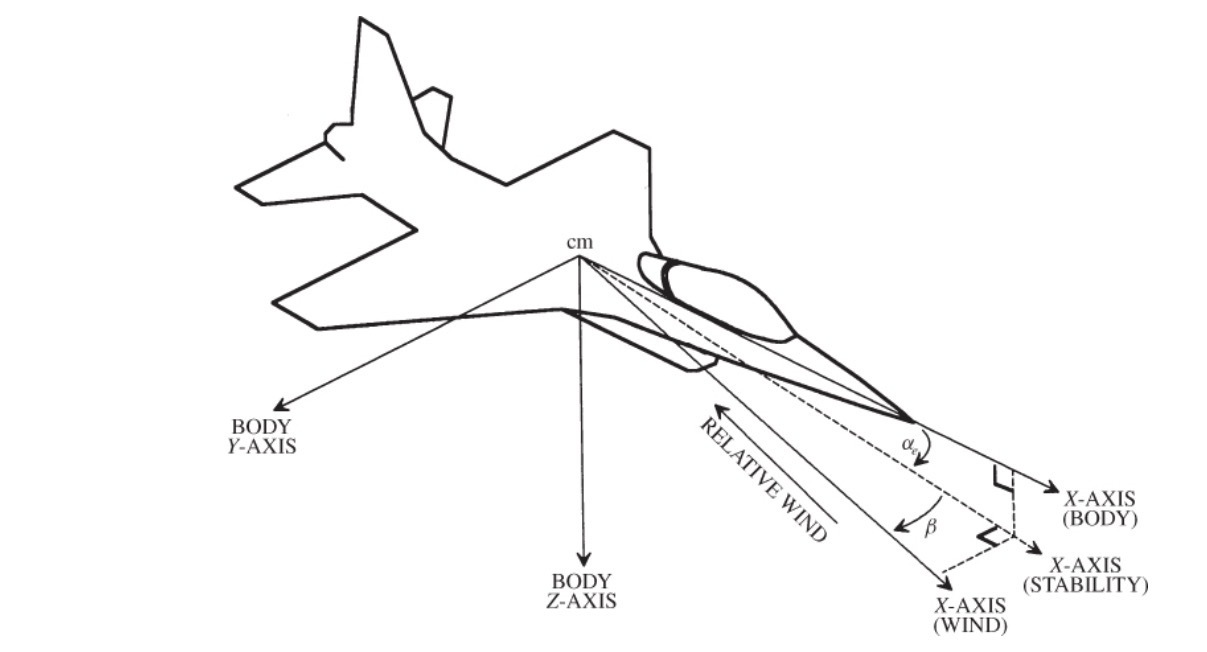
\includegraphics[width=0.7\linewidth]{Foto/photo/sistemi_riferimento}
    	\caption{Definizione dei sistemi di coordinate: la terna solidale al velivolo (Body Frame - FRD) e la terna inerziale terrestre (Earth Frame - NED).}
    	\label{fig:sistemiriferimento}
    \end{figure}
    \item \textbf{Target Plane ($tp$):} Piano di destinazione inerziale utilizzato per la navigazione. I vettori atmosferici vengono spesso definiti in questo sistema.
    
    \item \textbf{Body Frame ($bf$ o $frd$) - Convenzione FRD:} Sistema di riferimento non inerziale con origine nel baricentro (\textit{Center of Mass}, CM) del velivolo. Gli assi seguono la convenzione \textbf{FRD} (\textit{Forward, Right, Down}):
    \begin{itemize}
        \item $X_{frd}$: Asse longitudinale, punta verso il muso (\textit{Forward}).
        \item $Y_{frd}$: Asse trasversale, punta verso l'ala destra (\textit{Right}).
        \item $Z_{frd}$: Asse verticale, punta verso la pancia (\textit{Down}).
    \end{itemize}

    \item \textbf{Wind Frame ($w$):} Sistema di riferimento allineato con il vettore della velocità relativa dell'aria.
    
    \item \textbf{Stability Frame ($s$):} Sistema di riferimento intermedio, allineato con la proiezione della velocità relativa sul piano di simmetria del velivolo.
\end{itemize}

\begin{table}[H]
	\centering
	\footnotesize
	\renewcommand{\arraystretch}{1.1}
	\begin{tabular}{p{0.15\textwidth} p{0.6\textwidth} p{0.15\textwidth}}
		\toprule
		\textbf{Simbolo} & \textbf{Descrizione} & \textbf{Unità} \\
		\midrule
		$V_T$ & Velocità vera del velivolo rispetto alla massa d'aria (\textit{True Airspeed}) & [m/s] \\
		$\alpha$ & Angolo d'attacco (\textit{Angle of Attack}) & [rad] \\
		$\theta$ & Angolo di assetto longitudinale rispetto all'orizzonte (\textit{Pitch Angle}) & [rad] \\
		$q$ & Velocità angolare di beccheggio in assi corpo (\textit{Pitch Rate}) & [rad/s] \\
		$h$ & Quota altimetrica del velivolo (\textit{Altitude}) & [m] \\
		$a_z$ & Accelerazione specifica misurata lungo asse Z, usata come feedback primario & [m/s$^2$] \\
		$\delta_{th}$ & Comando di manetta (\textit{Throttle}) & [0 - 1] \\
		$\delta_e$ & Deflessione del piano di coda orizzontale (\textit{Elevator}) & [rad] \\
		$T$ & Spinta del turbofan (\textit{Thrust}) & [N] \\
		$m$ & Massa del velivolo & [kg] \\
		$g$ & Accelerazione di gravità & [m/s$^2$] \\
		$\bar{q}$ & Pressione dinamica & [Pa] \\
		$S$ & Superficie alare & [m$^2$] \\
		$\bar{c}$ & Corda media aerodinamica & [m] \\
		$I_{yy}$ & Momento d'inerzia di beccheggio & [kg$\cdot$m$^2$] \\
		$C_D, C_L, C_m$ & Coefficienti di Resistenza, Portanza e Momento & [-] \\
		$C_{m_q}$ & Smorzamento aerodinamico derivato dalla rotazione $q$ & [-] \\
		$\Delta C_{m_{cg}}$ & Correzione del momento di beccheggio causata dal baricentro (\textit{CG}) & [-] \\
		\bottomrule
	\end{tabular}
	\caption{Legenda e Significato Fisico delle Variabili del Moto Longitudinale}
	\label{tab:longitudinal_vars}
\end{table}

\section{Vettori di stato e cinematica del vento}
\subsection*{Vettore di Stato Globale ($\mathbf{X}$)}


La dinamica a 6 gradi di libertà è descritta dal \textbf{vettore di stato globale $\mathbf{X} \in \mathbb{R}^{12}$}.
\begin{equation}
\mathbf{X} = 
\begin{bmatrix}
\bm{\Phi} \\
\boldsymbol{\omega}_{b/e}^{frd} \\
\mathbf{V}_{cm/e}^{frd} \\
\mathbf{P}^E
\end{bmatrix}
=
\begin{bmatrix}
\phi \\ \theta \\ \psi \\ p \\ q \\ r \\ u \\ v \\ w \\ p_N \\ p_E \\ p_D
\end{bmatrix}
\end{equation}
Dalla componente verso il basso ($p_D$), si definisce la quota altimetrica $h$ e il rateo di salita:
\begin{equation}
\dot{h} = -\dot{p}_D
\end{equation}

\subsection*{Vettori Atmosferici e Cinematica del Vento}
Si definisce il vettore velocità del vento misurato nel Target Plane:
\begin{equation}
\mathbf{V}_{w/e}^{tp} = \begin{bmatrix} W_N \\ W_E \\ W_D \end{bmatrix}
\end{equation}

Per ricavare la velocità relativa dell'aria nel sistema FRD ($\mathbf{V}_r^{frd}$), si proietta il vento tramite la matrice dei coseni direttori (\textit{Direction Cosine Matrix}, DCM) $\mathbf{C}_{frd/tp}$, scritta con la notazione compatta:
\begin{equation}
\mathbf{C}_{frd/tp} = 
\begin{bmatrix}
c\theta c\psi & c\theta s\psi & -s\theta \\
s\phi s\theta c\psi - c\phi s\psi & s\phi s\theta s\psi + c\phi c\psi & s\phi c\theta \\
c\phi s\theta c\psi + s\phi s\psi & c\phi s\theta s\psi - s\phi c\psi & c\phi c\theta
\end{bmatrix}
\end{equation}

La velocità relativa del velivolo è quindi:
\begin{equation}
\mathbf{V}_r^{frd} = \mathbf{V}_{cm/e}^{frd} - \mathbf{C}_{frd/tp} \mathbf{V}_{w/e}^{tp}
\end{equation}



\section{Modellazione di forze e momenti aerodinamici}

\subsection{Forze nel Body Frame ($bf$)}
Le forze esterne nel sistema Body si suddividono in effetti aerodinamici ($A$) ed effetti propulsivi o di spinta ($T$, \textit{Thrust}):
\begin{equation}
\mathbf{F}_A^{bf} = \begin{bmatrix} X_A \\ Y_A \\ Z_A \end{bmatrix}, \quad \mathbf{F}_T^{bf} = \begin{bmatrix} X_T \\ Y_T \\ Z_T \end{bmatrix}
\end{equation}
dove $X_A, Y_A, Z_A$ rappresentano l'effetto aerodinamico puro, e $X_T, Y_T, Z_T$ la forza propulsiva.

\subsection{Forze nel Wind Frame ($w$)}
Nel sistema del vento ($w$), le forze aerodinamiche assumono la loro denominazione classica: Resistenza ($D$, \textit{Drag}), Forza Laterale o Vento al Traverso ($C$, \textit{Cross Wind force}) e Portanza ($L$, \textit{Lift}). Rispettando l'orientamento degli assi, il vettore è definito come:
\begin{equation}
\mathbf{F}_A^w = \begin{bmatrix} -D \\ -C \\ -L \end{bmatrix}
\end{equation}

La relazione matematica che proietta gli effetti aerodinamici dal Body Frame al Wind Frame utilizza la matrice di trasformazione $\mathbf{C}_{w/bf}$ (funzione di incidenza $\alpha$ e derapata $\beta$):
\begin{equation}
\mathbf{F}_A^w = \begin{bmatrix} -D \\ -C \\ -L \end{bmatrix} = \mathbf{C}_{w/bf} \begin{bmatrix} X_A \\ Y_A \\ Z_A \end{bmatrix}
\end{equation}

\subsection{Momenti Aerodinamici}
I momenti aerodinamici attorno al baricentro sono raggruppati in un vettore colonna contenente i ratei di rollio ($l$), beccheggio ($m$) e imbardata ($n$):
\begin{equation}
\mathbf{M} = \begin{bmatrix} l \\ m \\ n \end{bmatrix}
\end{equation}
È di cruciale importanza notare che i valori delle componenti cambiano a seconda del sistema di riferimento in cui il vettore viene espresso:
\begin{itemize}
    \item $\mathbf{M}_A^bf= [l^{bf}, m^{bf}, n^{bf}]^T$: Momenti nel Body Frame.
     \item $\mathbf{M}_A^s = [l^{s}, m^{s}, n^{s}]^T$: Momenti negli Assi di Stabilità.
     \item $\mathbf{M}_A^w = [l^{w}, m^{w}, n^{w}]^T$: Momenti negli Assi Vento.
\end{itemize}
All'interno del codice di simulazione, i momenti dimensionali vengono estratti scalando i \textbf{coefficienti di momento adimensionali} ($C_l, C_m, C_n$) ricavati dal database aerodinamico.

